\subsection{Embedding: Complemented Type System Lattice}

{  \setbeamercolor{background canvas}{bg=sectioncolor}
\begin{frame}{\Challenge{2} Type Lattice}

  How to support types like \textcolor{greeny}{$Int\cap\overline{Number}$} in Clojure, Scala, Python?

  Similar to that build-in to  Common Lisp.

  %% \begin{itemize}
  %% \item Support \Emph{complemented type lattice}
  %% \item SETS: Simple Embedded Type System
  %% \item Embed a dynamic type system into an existing programming language.
  %% \item Support application-specific predidate as type. \Eg \code{oddp}, \code{negativep}
  %% \item Answer type membership and subtype questions.
  %% \end{itemize}

\end{frame}
}

\begin{frame}{Simple Embedded Type System: SETS}

  \begin{itemize}
  \item Wrap/embed the PL-built-in type system
  \item ... with a \Emph{simple} type system
  \item ... which supports a complemented \Emph{type lattice}
  \item ... with \Emph{membership Boolean} predicate
  \item ... with \Emph{subtype semi-Boolean} predicate
  \item ... which supports \Emph{reflection}
  \end{itemize}

\end{frame}


\newsavebox\tdast
\begin{lrbox}{\tdast}
  \begin{minipage}{11cm}
    %% dont re-indent this file
\begin{lstlisting}[style=reclojureScala]
val Int      = SAtomic(classOf[Int])
val Double = SAtomic(classOf[Double])
val td:SimpleTypeD = SOr(Double, SAnd(Int, SNot(SEql("X"))))
\end{lstlisting}

  \end{minipage}
\end{lrbox}


\begin{frame}{Type Designator Expression Tree: AST}
  \centering

  \scalebox{0.95}{% Modeled after the following
% A simple Tree
% Author: Stefan Kottwitz
% https://www.packtpub.com/hardware-and-creative/latex-cookbook
\documentclass[border=10pt]{standalone}
\usepackage{tikz}
\begin{document}
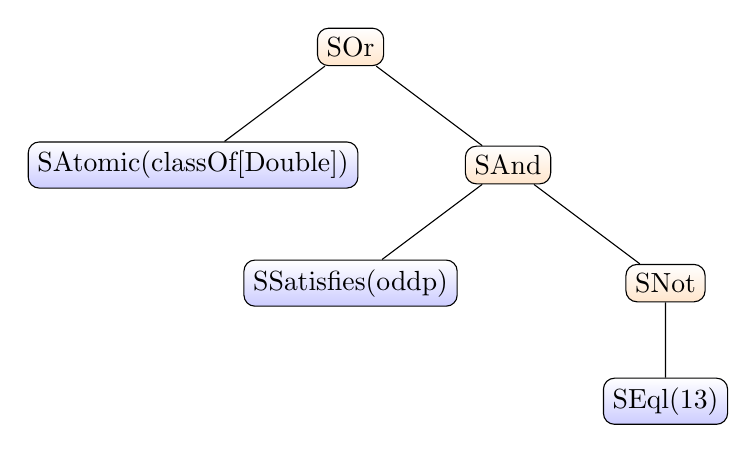
\begin{tikzpicture}[sibling distance=10em,
  every node/.style = {shape=rectangle, rounded corners,
    draw, align=center,
    top color=white, bottom color=orange!20}]]
    \tikzstyle{level 1}=[sibling distance=40mm]
    \tikzstyle{level 2}=[sibling distance=40mm]
    \tikzstyle{level 3}=[sibling distance=40mm]
  \node {SOr}
    child { node [bottom color=blue!20] {SAtomic(classOf[Double])} }
    child { node {SAnd}
      child { node [bottom color=blue!20] {SSatisfies(oddp)} }
      child { node {SNot} 
        child { node [bottom color=blue!20] {SEql(13)} } } } ;
\end{tikzpicture}
\end{document}
}

\end{frame}



\newsavebox\membershipbox
\begin{lrbox}{\membershipbox}
  \begin{minipage}{11cm}
    %% dont re-indent this file
\begin{lstlisting}[style=reclojureClojure]
;; returns true
(typep -42 'Integer)

;; returns true
(typep 7 '(or String Integer))

;; returns false
(typep 32 '(satisfies odd?))
\end{lstlisting}

  \end{minipage}
\end{lrbox}

\begin{frame}{Type Membership Predicate}{$x \in \tysem{\typevar} \to \{true, false\}$}
  \Emph{Boolean} membership question is \Emph{always answerable}.

  \usebox\membershipbox
\end{frame}

\newsavebox\subtypebox
\begin{lrbox}{\subtypebox}
  \begin{minipage}{11cm}
%% dont re-indent this file
\begin{lstlisting}[style=reclojureScala]
val Str:SimpleTypeD = SAtomic(classOf[String])
val Int:SimpleTypeD = SAtomic(classOf[Int])
val Num:SimpleTypeD = SAtomic(classOf[Number])
val odd:SimpleTypeD = SSatisfies(oddp, "oddp")

Int.subtypep(Num)  // returns Some(true) -- Yes
Str.subtypep(Int)  // returns Some(false) -- No
SSatisfies(oddp).subtypep(Int) // returns None -- Dont-know
\end{lstlisting}

  \end{minipage}
\end{lrbox}



\begin{frame}{Subtype Predicate}{$\tysem{\typevar}\subset\tysem{\typevart} \to \{true,false,\text{dont-know}\}$}
  \begin{itemize}
    
  \item   \Emph{Semi-Boolean} Subtype predicate \Emph{sometimes unanswerable}.
    
    \usebox\subtypebox
    
  \item Unanswerable because:
    \begin{itemize}
    \item Impossible to compute, \eg \code{satisfies}.
    \item Code is incomplete.
    \item Loading classes at run-time.
    \end{itemize}
    
  \item Determine habitation/vacuity
    \begin{itemize}
    \item $A \subset \emptyset$
    \end{itemize}

  \item Determine disjointness
    \begin{itemize}
    \item Disjoint:  $A \subset \compl{B}$
    \item Disjoint: $A\cap B \subset \emptyset$
    \end{itemize}
  \end{itemize}
  
\end{frame}

